% Asset ID: AS1DifferentiationTIKZ-009
% Source: Chapter 12 optimisation tank evidence + CCEA AS1-DIFF-LO007
% Related lesson section: Core Theory 25
% Purpose: Show open-top cuboid tank with square opposite faces and dimensions x and y.

\documentclass[tikz,border=8pt]{standalone}
\usepackage{amsmath}
\usetikzlibrary{arrows.meta}

\begin{document}
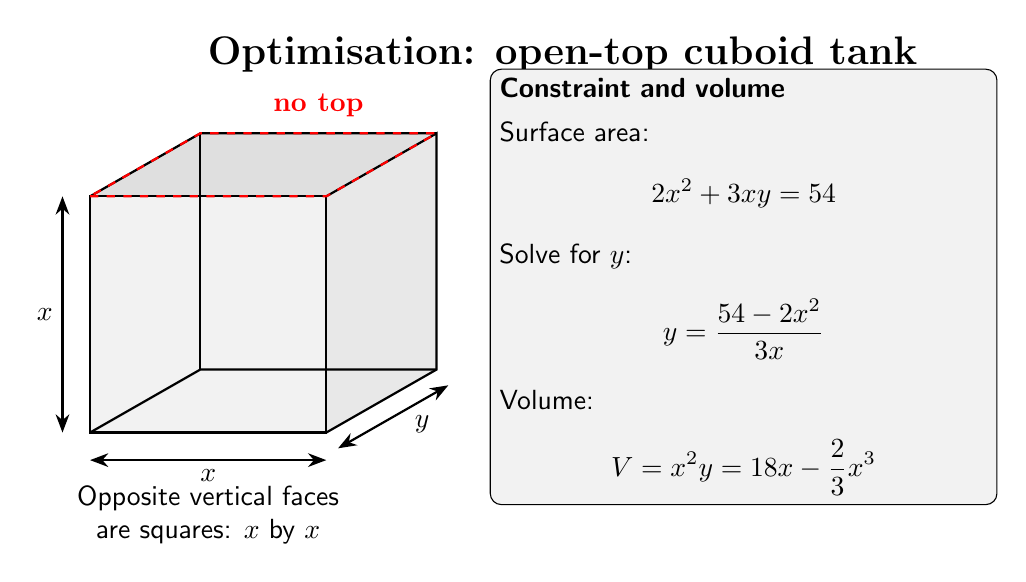
\begin{tikzpicture}[font=\sffamily, >=Stealth]

\node[font=\Large\bfseries] at (6,4.8) {Optimisation: open-top cuboid tank};

\coordinate (A) at (0,0);
\coordinate (B) at (3,0);
\coordinate (C) at (3,3);
\coordinate (D) at (0,3);
\coordinate (E) at (1.4,0.8);
\coordinate (F) at (4.4,0.8);
\coordinate (G) at (4.4,3.8);
\coordinate (H) at (1.4,3.8);

\fill[gray!10] (A)--(B)--(C)--(D)--cycle;
\fill[gray!18] (B)--(F)--(G)--(C)--cycle;
\fill[gray!25] (D)--(C)--(G)--(H)--cycle;

\draw[thick] (A)--(B)--(C)--(D)--cycle;
\draw[thick] (B)--(F)--(G)--(C);
\draw[thick] (D)--(H)--(G);
\draw[thick] (A)--(E)--(F);
\draw[thick] (E)--(H);

\draw[red, thick, dashed] (D)--(C)--(G)--(H)--cycle;
\node[red, font=\bfseries] at (2.9,4.15) {no top};

\draw[<->, thick] (-0.35,0) -- (-0.35,3);
\node[left] at (-0.35,1.5) {$x$};

\draw[<->, thick] (0,-0.35) -- (3,-0.35);
\node[below] at (1.5,-0.35) {$x$};

\draw[<->, thick] (3.15,-0.2) -- (4.55,0.6);
\node[right] at (4.0,0.1) {$y$};

\node[align=center] at (1.5,-1.05) {Opposite vertical faces\\are squares: $x$ by $x$};

\node[draw, rounded corners, fill=gray!10, align=left, text width=6.2cm] at (8.3,1.85)
{
\textbf{Constraint and volume}\\[4pt]
Surface area:
\[
2x^2+3xy=54
\]
Solve for \(y\):
\[
y=\frac{54-2x^2}{3x}
\]
Volume:
\[
V=x^2y=18x-\frac23x^3
\]
};

\end{tikzpicture}
\end{document}
